\documentclass[tikz]{standalone}
\usepackage{tikz}
\usetikzlibrary{patterns,snakes}
 
\begin{document}
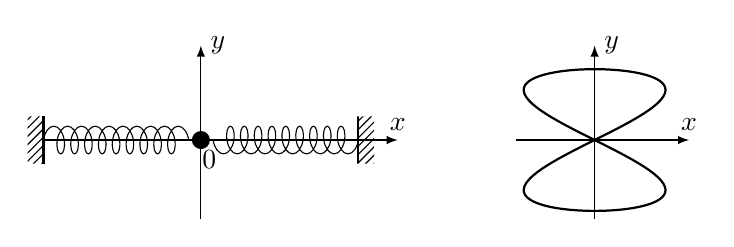
\begin{tikzpicture}
	\draw [arrows={-latex}] (-2,0) -- (2.5,0) node [above] {$x$};
	\draw [arrows={-latex}] (0,-1) -- (0,1.2) node [right] {$y$};
	\draw [snake=coil, segment amplitude=5pt, segment length=5pt] (-2,0) -- (0, 0);
	\draw [snake=coil, segment amplitude=5pt, segment length=5pt] (2,0) -- (0, 0);
	\draw [thick] (-2,-0.3) -- (-2,0.3) (2,-0.3) rectangle (2,0.3);
	\draw [draw=none, pattern=north east lines] (-2.2,-0.3) rectangle (-2,0.3) 
											   (2.2,-0.3) rectangle (2,0.3);
	\draw [thick, fill] (0, 0) circle (0.1) node [right=3pt,below] {$0$};
	\draw [arrows={-latex}] (4,0) -- (6.2,0) node [above] {$x$};
	\draw [arrows={-latex}] (5,-1) -- (5,1.2) node [right] {$y$};
	\draw [thick, parametric, domain=-3.14:3.14, samples=200, variable=\t] plot ({0.9*sin(2*\t r)+5},{0.9*sin(\t r)});
\end{tikzpicture}
\end{document}